\chapter{Конструкторская часть}

В этом разделе будут представлены требования к программному обеспечению (ПО), схема и трудоемкость алгоритмов.

\section{Требования к программному обеспечению}

Программе передается массив в качестве входных данных, а на выход получается отсортированный массив. 
Кроме того, необходимо сообщить пользователю затраченное каждым алгоритмом процессорное время и  используемая память.

В создаваемом приложении пользователю должны быть доступны функции ввода элементов массива и выбора желаемого алгоритма. 

\section{Разработка алгоритма соритовки слиянием}

На рисунке \ref{fig:merge_sort} приведена схема рассматриваемого алгоритма.
\FloatBarrier
\begin{figure}[h]
	
	\centering{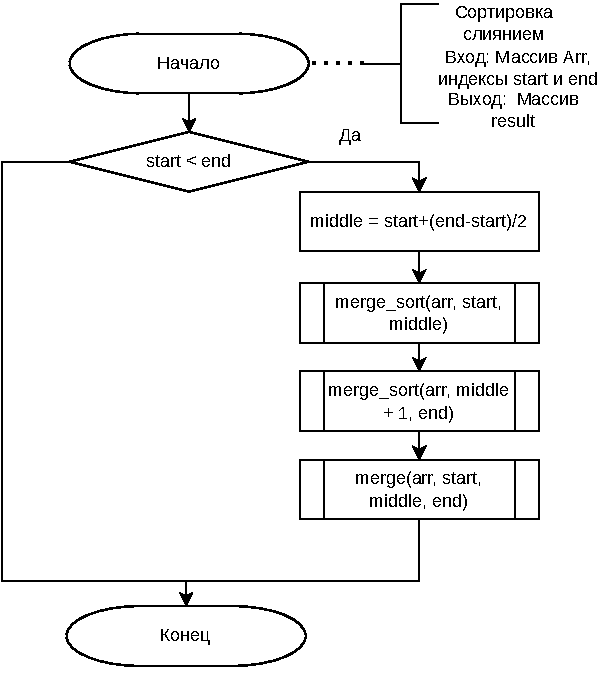
\includegraphics[scale=0.69]{photos/merge_sort.pdf}}
	
	\caption{Схема алгоритма сортировки слиянием}
	
	\label{fig:merge_sort}
\end{figure}
\FloatBarrier
\clearpage

\section{Разработка алгоритма сортировки бинарным деревом}

На рисунке \ref{fig:bin_tree} приведена схемa рассматриваемого алгоритма.
\FloatBarrier
\begin{figure}[h]
	
	\centering{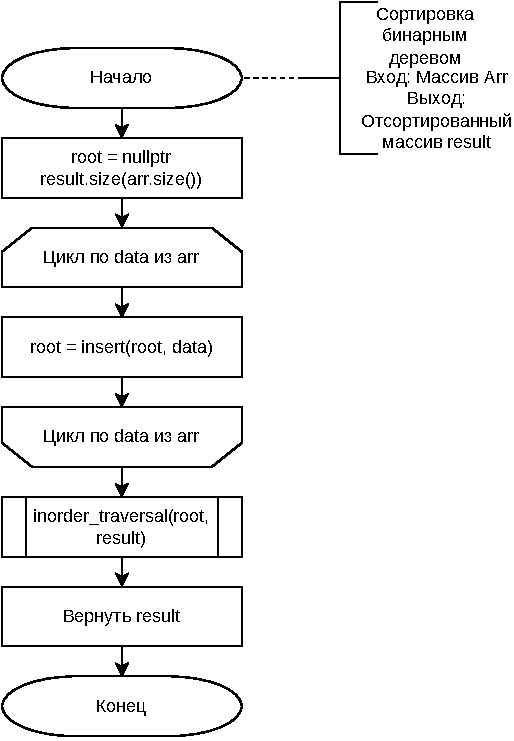
\includegraphics[scale=1]{ photos/bin_tree.pdf}}
	\caption{Схема алгоритма сортировки бинарным деревом}
	\label{fig:bin_tree}
\end{figure}
\FloatBarrier
\clearpage

\section{Разработка алгоритма сортировки расчесткой}

На рисунке \ref{fig:coctail_sort} приведена схемa рассматриваемого алгоритма.
\FloatBarrier
\begin{figure}[h]
	\centering{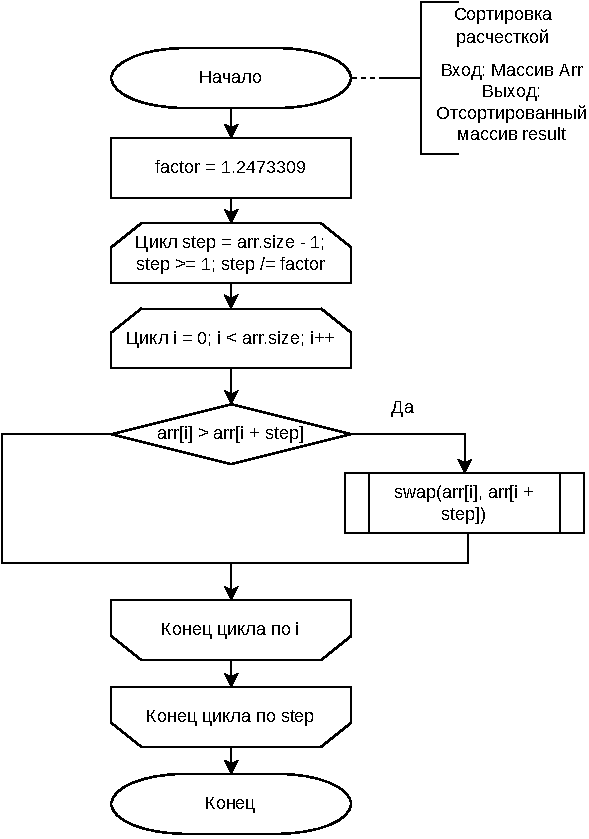
\includegraphics[scale=1]{photos/coctail_sort.pdf}}
	\caption{Схема алгоритма сортировки расчесткой}
	\label{fig:coctail_sort}
\end{figure}
\FloatBarrier
\clearpage

\section{Модель вычислений}
Для дальнейшего анализа трудоемкости необходимо ввести модель вычислений.

Операции из списка (\ref{for:opers}) имеют трудоемкость 1.

\begin{equation}
	\label{for:opers}
	=, +=, -=, +, -, ==, !=, <, >, <=, >=, [], ++, {-}-
\end{equation}

Операции из списка (\ref{for:opers2}) имеют трудоемкость 2.
\begin{equation}
	\label{for:opers2}
	*, /, \%
\end{equation}

Трудоемкость оператора выбора \code{if условие then A else B} рассчитывается как:
\begin{equation}
	\label{for:if}
	f_{if} = f_{\text{условия}} +
	\begin{cases}
		f_A, & \text{если условие выполняется,}\\
		f_B, & \text{иначе.}
	\end{cases}
\end{equation}

Трудоемкость цикла рассчитывается как:
\begin{equation}
	\label{for:for}
	f_{for} = f_{\text{инициализации}} + f_{\text{сравнения}} + N(f_{\text{тела}} + f_{\text{инкремента}} + f_{\text{сравнения}})
\end{equation}

Трудоемкость вызова функции равна 0.

\section{Трудоемкость алгоритмов}
Далее размер массива обозначаетсй как size.

\subsection{Алгоритм сортировки слиянием}
Трудоемкость алгоритма сортировки слиянием состоит из:

\begin{itemize}
	\item рекурсивное разбиение массива на массивы половинной длины:
	\begin{equation}
		\label{worst_counting}
		f_{\text{разбиение}} = log_2{(size)}
	\end{equation}
	
	\item трудоемкость соединения двух массивов половинной длины:
	\begin{equation}
		\label{worst_counting}
		f_{\text{соединение}} = 2 + size \cdot (3 + \begin{cases}
			4, & \text{в лучшем случае},\\
			10, & \text{в худшем случае}.\\
		\end{cases}
	\end{equation}
\end{itemize}

\subsection{Алгоритм сортировки бинарным деревом}

Трудоемкость алгоритма сортировки бинарным деревом состоит из:

\begin{itemize}
	\item Трудоемкости построения бинарного дерева, которая равна (\ref{make_tree}).
	\begin{equation}
		\label{make_tree}
		f_{make\_tree} = (5 \cdot \log(N) + 3) * N = N \cdot \log(N)
	\end{equation}
	\item Трудоемкости восстановления порядка элементов массива, которая равна (\ref{make_arr}):
	\begin{equation}
		\label{make_arr}
		f_{main\_loop} = 7 N
	\end{equation}
\end{itemize}

Таким образом общая трудоемкость алгоритма выражается как (\ref{for:been_total}).

\begin{equation}
	\label{for:been_total}
	f_{total} = f_{make\_tree} + f_{main\_loop}
\end{equation}

Трудоемкость алгоритма в лучшем случае (\ref{been_min}).

\begin{equation}
	\label{been_min}
	f_{best} = O(N\log(N))
\end{equation}

Трудоемкость алгоритма в худшем случае (\ref{been_max}).

\begin{equation}
	\label{been_max}
	f_{worst} = O(N\log(N))
\end{equation}

Трудоёмкость в лучшем случае (массив отсортирован):

\begin{equation}
	\begin{array}{cc}
		f_{\text{лучший}} = log_2(size) \cdot (2 + size \cdot 7) \approx  size \cdot log_2(size) =\\ O(size \cdot log_2(size))  
	\end{array}
\end{equation}
\pagebreak

Трудоёмкость в худшем случае (массив отсортирован в обратном порядке):

\begin{equation}
	\begin{array}{cc}
		f_{\text{худший}} = log_2(size) \cdot (2 + size \cdot 13) \approx  size \cdot log_2(size) = \\O(size \cdot log_2(size))             
	\end{array}
\end{equation}

Трудоемкость в худшем и лучшем случае равна $O(size \cdot log_2(size))$.

\subsection{Алгоритм сортировки расчесткой}
Трудоемкость алгоритма сортировки расчёсткой может быть оценена следующим образом:

Трудоемкость алгоритма в лучшем случае (\ref{combo_max}).
\begin{equation}
	\label{combo_max}
	f_{best} = O(size\log(size))
\end{equation}

Трудоемкость алгоритма в худшем случае (\ref{combo_min}).
\begin{equation}
	\label{combo_min}
	f_{worst} = O(size^{2})
\end{equation}

\section*{Вывод}

На основе теоретических знаний, полученных в аналитическом разделе, были разработаны схемы алгоритмов, благодаря которым может быть упорядочено множество объектов разными способами. 
Также для каждого из них были рассчитаны и оценены лучшие и худшие случаи.
